%! Author = nico
%! Date = 20.05.23

\section{Randbedingungen}
\label{sec:randbedingungen}
Der Entwurf des Systems wird leicht durch das bereits existierende System eingeschränkt. Die Datenstruktur der zu
verkaufenden Biere ist bereits gegeben und sieht folgendermassen aus:
\begin{figure}[H]
    \centering
    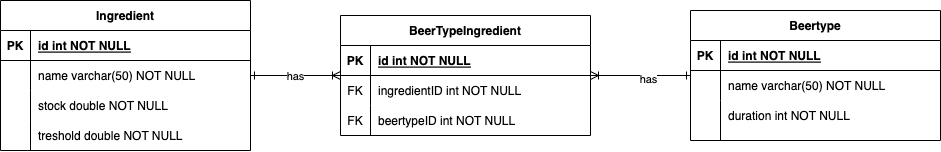
\includegraphics[width=1.0\textwidth]{../images/kontextabgrenzung/PA5-Datenstruktur.png}
    \caption{Datenstruktur der Biere}
    \label{fig:randbedingungen}
\end{figure}

Für die Datenstruktur eines Produkts, das auf der Webseite angezeigt wird, müssen sicherlich noch einige Ergänzungen an der
Datenstruktur vorgenommen werden, beispielsweise fehlt aktuell pro Produkt die Anzahl der verfügbaren Einheiten.

Die Datenstrukturen der Kunden und der Bestellungen sind noch nicht vorhanden und können frei gestaltet werden.

Ebenfalls ist durch die technische Aufgabenstellung der Einsatz einer serviceorientierten Architektur und von 
verschiedenen Technologien vorgegeben. Dazu gehören JakartaEE, Spring Boot, Micronaut, Docker und Kubernetes. 
Die Anzahl der zu entwerfenden Services beläuft sich also auf mindestens drei. Ebenfalls gilt es, eine Datenbank
zu verwenden, welche die Daten der Produkte, Kunden und Bestellungen speichert. Die Datenbank kann frei gewählt werden.
Um die gesamte Logik sinnvoll zu präsentieren, muss ebenfalls eine Benutzeroberfläche entworfen werden. Auch hierbei
steht die Technologie frei.
